\section{Theorie \cite{sample}}

\textbf{\underline{Ziel:}}
Im ersten Teil des Versuches sollen die Schwingungen in ihre Fourierkomponenten zerlegt werden.
Daufhin sollen eben diese Schwingungen im zweiten Teil des Versuches aus Oberwellen erzeugt werden.

\subsection{Fouriersches Theorem}

Ist eine Funktion periodisch, so gilt:
\begin{equation}
  f(x)=f(x+D)
\end{equation}
für räumliche  und
\begin{equation}
  f(t)=f(t+T)
\end{equation}
für zeitliche periodische Vorgänge.
Wichtige periodische Funktionen sind die Sinus- und Cosinusfunktion.
Diese sind $2\pi$-periodisch und decken den Wertebereich von $-1$ bis $1$ ab.
Ebenso lassen sich durch
\begin{align}
  f(t) &=a \cdot \sin{(\frac{2\pi}{T}\cdot t)}  \\
  g(t) &=b \cdot \cos{(\frac{2\pi}{T}\cdot t)}
\end{align}
nahezu alle periodischen Vorgänge beschreiben, was aus dem Fourierschen Theorem folgt.
Dieses besagt, dass die Reihe
\begin{equation}
  f_\text{n}(x) = \frac{1}{2}a_0 + \sum_{n=1}^{\infty}\left(a_n \cos{(\frac{2\pi}{T}t)} + b_n \sin{(\frac{2\pi}{T}t)} \right)
  \label{eqn:FT}
\end{equation}
eine periodische Funktion f darstellt, wenn (\ref{eqn:FT}) konvergiert.
Ebenso ist zu erkennen, dass neben der Grundfrequenz $\nu_1 = 1/T$ nur ganzzahlige Vielfache
von $\nu_1$ - die sogenannten Oberschwingungen - auftreten.

\subsection{Fourier-Analyse}
Die in (\ref{eqn:FT}) enthaltenen Koeffizienten $a_n$ und $b_n$ lassen sich durch
\begin{align}
  a_n &= \frac{2}{T}\int\limits_{0}^T f(t)\cos{(\frac{2\pi}{T}t)}dt  \label{eqn:an} \\
  b_n &= \frac{2}{T}\int\limits_{0}^T f(t)\sin{(\frac{2\pi}{T}t)}dt  \label{eqn:bn}
\end{align}
bestimmen.
Die Bestimmung der Koeffizienten wird auch als Fourier-Analyse bezeichnet.
Es existieren jedoch zwei Spezialfälle, die die Rechnung vereinfachen:
\begin{itemize}
  \item Ist $f(t)$ gerade, also ist $f(t)=f(-t)$, so ist $b_n=0$.
    \item Ist $f(t)$ ungerade, also ist $f(t)=-f(-t)$, so ist $a_n=0$.
\end{itemize}
Werden die Amplituden der Teilschwingungen gegen die Frequenz aufgetragen,
so ergibt sich ein Linienspektrum wie in Abbildung \ref{fig:linie}.
\begin{figure}[H]
  \centering
  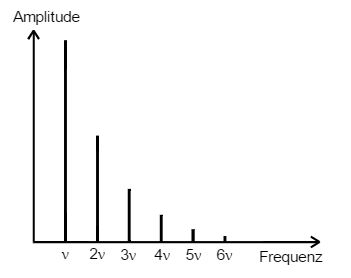
\includegraphics{Text/Bilder/linie.jpg}
  \caption{Linienspektrum \cite[271]{sample}}
  \label{fig:linie}
\end{figure}
Wird die Fourier-Analyse auf eine Funktion angewendet, die bei $f(t_\text{0})$ nicht stetig ist, so kann sie bei $t_\text{0}$
nicht appromixiert werden. Die daraus folgende Abweichung ist jedoch endlich.
Dies wird als Gibbsches Phänomen bezeichnet.

\subsection{Fourier-Transformation}
Während sich mit \eqref{eqn:an} und \eqref{eqn:bn} einzelne Komponenten einer periodischen Funktion bestimmen lassen,
so stellt
\begin{equation}
  g(\nu)=\int\limits_{-\infty}^\infty f(t)e^{i\nu t}dt \label{eqn:gnu}
\end{equation}
das gesamte Frequenzspektrum dar.
Bei einer periodischen Funktion besteht $g$ aus einer (konvergierenden) Reihe von $\delta$--Distributionen (siehe \ref{fig:linie}).
Diese Transformation ist auch umkehrbar. So ergibt sich für $f(t)$:
\begin{equation}
  f(t)=\frac{1}{2\pi}\int\limits_{-\infty}^\infty g(\nu)e^{-i\nu t}d\nu \label{eqn:ft}
\end{equation}
Allerdings werden bei \eqref{eqn:gnu} und \eqref{eqn:ft} über unendlich lange Zeiten bzw.
 unendlich viele Frequenzen integriert,
was in der Praxis nicht umsetzbar ist.
Dies hat zur Folge, dass Abweichungen zu den erwarteten Ergebnissen auftreten.
Ebenso folgt daraus, dass für $g$ keine Reihe von $\delta$-Distributionen erhalten wird,
sondern $g$ überall stetige und differenzierbare
Funktionen liefert. Des Weiteren treten Nebenmaxima auf, deren Amplituden jedoch schnell abnehmen.
